
\subsection{Lewin's Force Field Analysis}

	{A force field analysis was used to analyze the driving and restraining forces so as to decide whether DDE should consider outsourcing. Each force factor is ranked out of 5 in terms of significance and net sums of both the forces are calculated and compared to determine whether the change should occur.}
	
	\begin{figure}[H]
    	\centering
    	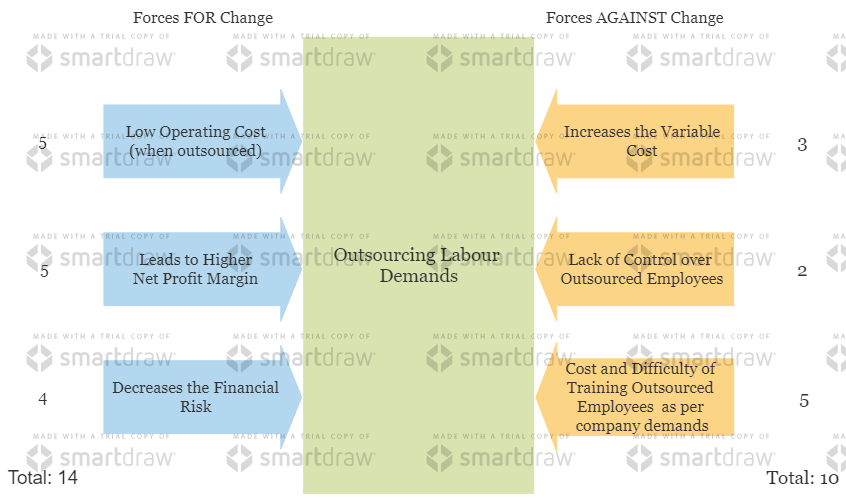
\includegraphics[width=15cm]{Lewin's Force Analysis.png}
    	%\caption{{Lewin's Force Field Analysis of the problem the company is facing}}
    	\label{}
	\end{figure}
	
	{The owner states that, his primary reasons for opting to outsource labour is because it would drastically drop the operating costs and that this move would to higher net profit margin; both of which can be evidently seen from the force field analysis as both of them rank those parameters as 5/5. Besides these forces that drive for the change within DDE to outsource labour, an another factor is that it reduces the financial risk within the company.}	
	
	{When evaluating the forces that act against the change, it is evident from the force field analysis that the major force against the move is the high cost and difficulty in training outsourced labour as per company demands and standards; While also the increase in variable cost and lack of authority \& control over the outsourced labour are also factors that are restraining the change.}
	
	{While comparing both the forces for and against the change we see that the driving forces exceed the restraining forces by 4 points which is significant enough to favor the change within DDE to outsource labour.}

\subsection{Ratio Analysis}

	{Ratio Analysis is a numerical and qualitative financial tool that can be used to determine the current and future financial position of DDE for if the company can consider outsourcing its labour demands.}

%	\noindent
%	% Gross Prift Margin (Current)
%	\begin{minipage}{.5\linewidth}
%	\begin{equation}
%		\frac{\text{Current Gross Proft}}{\text{Current Revenue}}\times 100 \%
%	\end{equation}
%	\end{minipage}
%	% Gross Profit Margin (Future)
%	\begin{minipage}{.5\linewidth}
%	\begin{equation}
%		\frac{\text{Predicted Gross Proft}}{\text{Predicted Revenue}}\times 100 \%
%	\end{equation}
%	\end{minipage}

	%	Gross Profit Margin (Current)

	$$\text{Gross Profit Margin (Current)} = \frac{\text{Current Gross Proft}}{\text{Current Revenue}}\times 100\% = \frac{\$1296000}{\$2160000}\times 100\% = 60\%$$

	%	Gross Profit Margin (Future)

	$$\text{Gross Profit Margin (Future)} = \frac{\text{Predicted Gross Proft}}{\text{Predicted Revenue}}\times 100\% = \frac{\$2333000}{\$3888000}\times 100\% \approx 60.2\%$$
	
	%	Net Profit Margin (Current)

	$$\text{Net Profit Margin (Current)} = \frac{\text{Current Net Profit}}{\text{Current Revenue}}\times 100\% = \frac{\$705375}{\$2160000}\times 100\% \approx 32.7\%$$
	
	%	Net Profit Margin (Future)

	$$\text{Net Profit Margin (Future)} = \frac{\text{Predicted Net Profit}}{\text{Predicted Revenue}}\times 100\% = \frac{\$1995000}{\$3888000}\times 100\% \approx 51.3\%$$
	
	%	Current Ratio (Only for Current)

	$$\text{Current Ratio} = \frac{\text{Current Assets}}{\text{Current Liabilities}} = \frac{\$600000}{\$245000} \approx 2.45$$
	
	%	Return on Capital Employed (Current)

	$$\text{Return on Capital Employed (Current)} = \frac{\text{NPBIT}}{\text{Capital Employed}}\times 100\% = \frac{\$897500}{\$699300}\times 100\% \approx 128\%$$
	
	%	Return on Capital Employed (Future)

	$$\text{Return on Capital Employed (Future)} = \frac{\text{NPBIT}}{\text{Capital Employed}}\times 100\% = \frac{\$2256000}{\$1731000}\times 100\% \approx 130\%$$

	{The Gross Profit Margin for both the company's current and predicted financial state (if the company is to decide to outsource its labour) are both relatively healthy and above the optimal $50\%$ range. This shows the company is profitable and has no issues with the lack of profitability. This statement is further supported by a very good Net Profit Margin of $32.7\%$ before considering outsourcing and an excellent predicted Net Profit Margin of $51.3\%$ after outsourcing.}
	
	{When analyzing the business Profit-Loss accounts, it is evident that other than the cost of revenue before outsourcing, the operating cost is relatively very high, whereas the operating cost after outsourcing is reduced significantly and is fraction of the original operating cost.}
	
	{The current ratio is largely positive, demonstrating that the company is in a healthy and stable Cash-Flow position and would not be at a financial risk if the company is to start outsourcing their labour demands.}	
	
	{We can confidently say from the above conclusions that the company can  increase their firm's growth and profit margin by outsourcing labour.}

\subsection{SWOT Analysis}

	{The internal strengths, weakness, opportunities as well as threats of the business were discussed with the owner and are included in the below SWOT analysis, which could help and aid us to decide if outsourcing labour is worth implementing.}
	
	\begin{figure}[H]
    	\centering
    	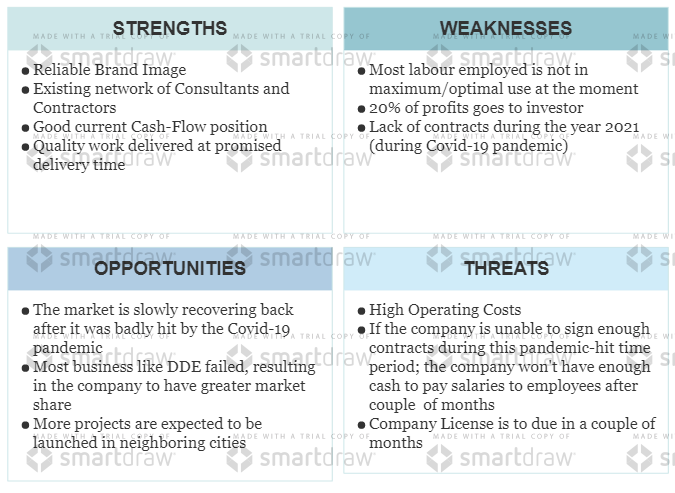
\includegraphics[width=15cm]{SWOT Analysis.png}
    	%\caption{{SWOT Analysis of the problem the company is facing}}
    	\label{}
	\end{figure}

	{The strengths of DDE are that it has a reliable brand image and has a good cash-flow position, whereas the major weakness of the business is that there is an insufficiency of projects in the year 2021 due the Covid-19 pandemic. The possible opportunities that the company can exploit are that market is slowly recovering from the economic backlash and current trends show that many projects are expected to be launched in neighboring cities, which DDE could possibly get contracts for, whereas the current threats that DDE encounters are the high operating costs and possible future issues related to cash-flow if future payments are not processed on time, as the company has enough money to sustain only a few months, without incoming payments.}	

\subsection{Fishbone Diagram}

	{The Fishbone diagram finds and analyses the root issue/problem faced within a business. This business tool shall determine the underlying problems/reasons faced by DDE causing the company to consider outsourcing. The main concern from the owner of the firm is Lower Profit Margin.}
	
	\begin{figure}[H]
    	\centering
    	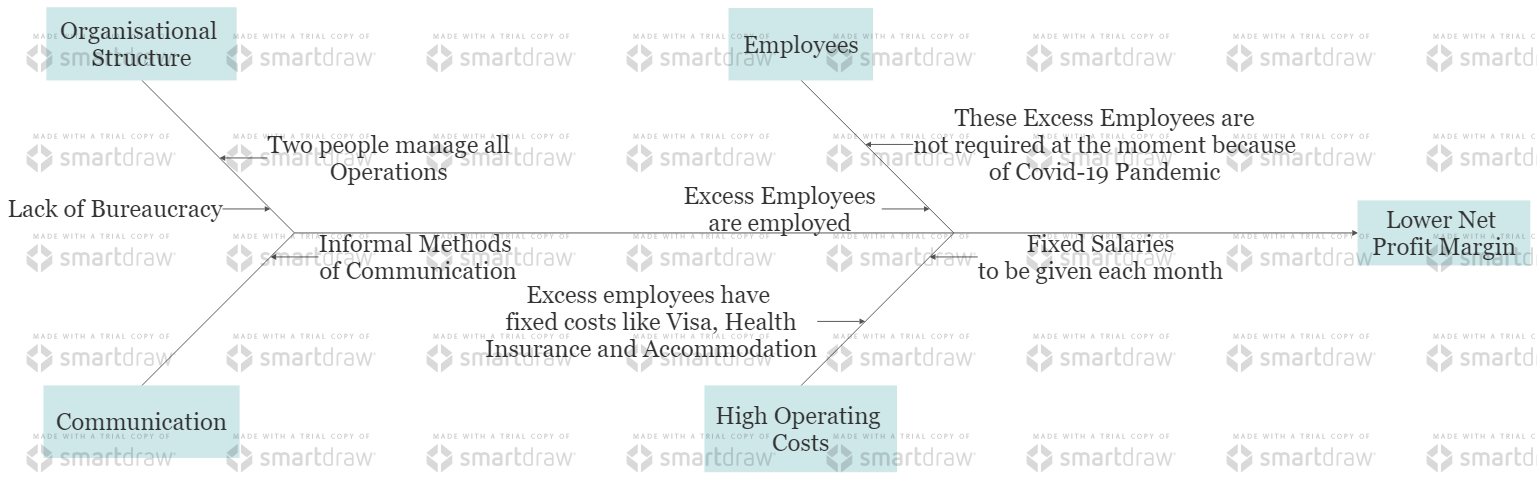
\includegraphics[width=15cm]{Fishbone Diagram.png}
    	%\caption{{Fishbone Diagram of the problem the company is facing}}
    	\label{}
	\end{figure}

	{The major issue of Lower Net Profit Margin that the company is facing is mainly High operating costs and Employees; both of which are due to the excess employees not required as the Covid-19 Pandemic hit the market. These employees are paid fixed salaries that increase fixed costs for the business.}
	
	{Other than these issues, the company has some serious internal issues regarding the organisational structure and communication within the company. This is because three people manage all company operations, and no supervisor/manager exists to overlook them. The employees use a very informal method of communication, namely, instant messaging over SMS or messaging apps like WhatsApp.}
	
	{All the above factors add up and result in causing the issue of reducing the company's Net Profit Margin drastically.}

%\subsection{PEST Analysis}

%	{}

